\documentclass[11pt]{article}
\usepackage[margin=1in]{geometry}
\usepackage[T1]{fontenc}
\usepackage{lmodern}
\usepackage{amsmath,amssymb}
\usepackage{booktabs}
\usepackage{graphicx}
\usepackage{xcolor}
\usepackage[numbers,sort&compress]{natbib}
\usepackage[colorlinks=true,linkcolor=blue!50!black,citecolor=blue!50!black,urlcolor=blue!50!black]{hyperref}

% ---- To fill after your git commits / tag (see README of the bundle) ----
\newcommand{\commitHyp}{\texttt{49883a9}}
\newcommand{\commitFrozen}{\texttt{9b0c42f}}
\newcommand{\commitResults}{\texttt{fc06f30}}
\newcommand{\repo}{\url{https://github.com/abdelkabirouadoukou/si-loop}}

\newcommand{\fh}{\texttt{final\_hard}}
\newcommand{\fa}{\texttt{final\_all}}
\newcommand{\auc}{\texttt{auc\_eval\_all}}

\title{A Controlled Ablation Study of a Guarded Self-Improvement Loop\\
with a Competitive Global Workspace in a Toy Setting}
\author{Abdelkabir Ouadoukou\thanks{Independent researcher. Contact: abdelkabir.ouadoukou@gmail.com.
This work was carried out with substantial AI assistance; see the disclosure at the end of the paper.}}
\date{November 2026 \\ \small Technical report (Study 1). Not peer reviewed.}

\begin{document}
\maketitle

\begin{abstract}
We study a small closed loop in which a hypernetwork emits adapters for a worker network, a learnability-driven
curriculum proposes tasks, a guarded judge accepts or rolls back each round, and a capacity-limited
\emph{competitive workspace} broadcasts selected training statistics back to the hypernetwork. The setting is a
synthetic few-shot sinusoid-regression family, run on CPU. We pre-specify four hypotheses and an analysis plan
(paired bootstrap, Bonferroni-adjusted intervals, a smallest effect of interest of $0.05$ in query MSE) and run four
arms (\texttt{full}, \texttt{no\_ws}, \texttt{random\_ws}, \texttt{no\_judge}) on ten paired seeds.
Results are mostly null or negative. We detect no difference between the competitive workspace and no workspace
(H1) or a random-winner workspace (H2); both comparisons have limited power (minimum detectable effects of about
$0.07$ and $0.06$). Removing the judge \emph{improved} final query MSE on the hard evaluation set by $0.086$
(Bonferroni 98.3\% CI $[-0.168,-0.014]$ on the \emph{arm minus full} difference), contradicting the expectation that the guards help (H3);
the judge accepted only about $27\%$ of rounds, so guarded arms received roughly four times fewer updates.
A Shapley-style interaction term was slightly larger in magnitude on rejected than accepted rounds (H4, small and confounded).
The toy has no adversarial pressure, so these results do \emph{not} show that judge guards are harmful in general.
We report the over-conservative judge, a curriculum that collapses to easy tasks, several post-hoc debugging steps and
dev-seed diagnostics performed before the report run, and the exact hashes needed to reproduce everything.
\end{abstract}

\section{Introduction and Related Work}

Recent work demonstrates pieces of self-improving systems in isolation: agents that rewrite their own code and
validate changes empirically \citep{zhang2025dgm,zhang2026hyperagents}, systems that mix harness rewrites with
weight updates \citep{hebbar2026sia}, models that generate their own finetuning data \citep{zweiger2025seal},
proposer/solver self-play with verifiable rewards \citep{zhao2025absolutezero}, and hypernetworks that emit
adapters from text or prompts \citep{charakorn2025t2l,liang2025dnd}. Surveys discuss the wider landscape of recursive
self-improvement \citep{chen2026rsi}. Evaluator exploitation is a known hazard: proxy-reward overoptimization
\citep{gao2023scaling,coste2024ensembles} and reward hacking of self-play judges \citep{zhou2026convincing}. Workspace-style
coordination, inspired by Global Workspace Theory \citep{baars1988cognitive}, has been proposed for LLM agents
\citep{shang2026theater} alongside blackboard architectures \citep{han2025blackboard}.

\paragraph{Question.} We ask a deliberately narrow, empirical question: in a toy loop where these ingredients are wired together,
(i) does a workspace that must \emph{select} what is shared help compared with no sharing or random sharing, and
(ii) do conservative judge controls help or hurt? The contribution is a pre-specified, fully reproducible ablation
with honest reporting of null and negative outcomes. It is \emph{not} a claim about recursive self-improvement, language models,
or scaling. Every component has prior art; we claim nothing about novelty of components.

\section{System Architecture}

\paragraph{Task family.} Each task is few-shot regression $y=a\sin(wx+p)$ with $a\sim U(0.5,2.5)$, with $K_{\text{sup}}=10$ support and
$K_{\text{qry}}=40$ query points. Predicting $0$ gives an MSE of about $1.29$ ($=\mathbb{E}[a^2]/2$), which is the reference level for ``no learning''.
The worker is a small MLP (hidden size $32$) with a low-rank adapter of rank $4$.

\paragraph{Loop.} Per round $t$: (1) the curriculum engine $C$ proposes tasks; (2) hypernetwork $A$ emits adapter parameters $\theta_A=(U,V,b_1,b_2)$ from the support set and
the workspace broadcast $g_t$; (3) worker $B$ adapts with $3$ inner SGD steps (learning rate $0.05$, gradient clipping at $5$);
(4) $A$ and $B$ are updated by a first-order meta-gradient of the query loss after adaptation (no second-order terms);
(5) $B$ and $C$ post summaries to the workspace $W$; (6) the judge $D$ decides acceptance.
On rejection, $A$, $B$, $C$ and their optimizers are rolled back to the last accepted snapshot.

\paragraph{Curriculum $C$.} A REINFORCE policy over $5$ difficulty bins with learnability reward $4\,s(1-s)$, where $s$ is the inner-loop success rate
under threshold $\tau=0.3$; this peaks at $50\%$ success.

\paragraph{Competitive workspace $W$.} Capacity $K=4$, ignition threshold $\theta=0.1$, time-to-live $4$ rounds, per-source posting limit $2$, typed numeric payloads.
Candidates compete on
\begin{equation}
\text{sal}=0.5\,\text{rel}+0.3\,\text{nov}+0.3\,\text{trust}\cdot\text{verified}+0.2\,\text{util}-0.3\,\frac{\text{age}}{\text{TTL}},
\end{equation}
and the broadcast $g_t$ is the mean of the winners' embeddings, where each embedding is a fixed $16$-dimensional random projection of scalar
training statistics (a stand-in for a semantic embedding). Consequently the workspace carries little information beyond random projections of scalar
training statistics, which is a boundary condition for interpreting H1 and H2. In \texttt{no\_ws} the broadcast is zeros; in \texttt{random\_ws} the capacity and TTL are identical but winners are chosen at random.
A rejected round retries under the \emph{last accepted} broadcast.

\paragraph{Credit assignment.} With old versions $(A_0,B_0)$ and candidate versions $(A,B)$, let $v(\cdot)=-\text{MSE}$ on a fixed diagnostic set
and write $v_0,v_A,v_B,v_{AB}$ for the four version combinations. The two-player Shapley values are
\begin{equation}
\varphi_A=\tfrac12\big[(v_A-v_0)+(v_{AB}-v_B)\big],\qquad
\varphi_B=\tfrac12\big[(v_B-v_0)+(v_{AB}-v_A)\big],
\end{equation}
so $\varphi_A+\varphi_B=v_{AB}-v_0$ exactly (efficiency; \citealp{shapley1953value}), and the interaction
$I=v_{AB}-v_A-v_B+v_0$ measures co-adaptation. $C$ is excluded because its effect flows through the data distribution.

\paragraph{Guarded judge $D$.} (i) \emph{Sealed randomness}: $A,B,C$ never access $D$'s generator. (ii) \emph{Fresh selection tasks} each round, in the spirit of
limiting adaptive reuse of a holdout \citep{dwork2015holdout}. (iii) \emph{Lower-confidence-bound gate}: accept only if $\overline{d}-\mathrm{sd}(d)/\sqrt{n}>0$ for paired per-task improvements $d$.
(iv) \emph{Gap monitor}: flag a round if the query-minus-support gap exceeds $\text{gap}_{\text{ema}}+0.25|\text{gap}_{\text{ema}}|+0.02$, where the EMA is updated only on accepted rounds.
(v) \emph{Hidden canary}: a held-out check released as one Laplace-noised bit ($\sigma=0.02$, margin $0.05\,c_{\text{old}}$, budget $200$ queries).
A round is accepted only if all controls pass. In \texttt{no\_judge} every round is accepted; the controls are still logged.

\section{Pre-Registration and Experimental Design}

\paragraph{Status of the pre-registration.} The hypotheses (\texttt{docs/hypotheses.md}) were written before the report run and are \emph{informal} (after the run, only the status line, the disclosure section and the deviations log were edited; the pre-run text is kept as \texttt{docs/hypotheses\_prerun.md}): there is no third-party registry timestamp. Their integrity rests on git commit order
(hypotheses and the dev-diagnostics disclosure at commit \commitHyp; frozen code tagged \texttt{frozen-config} at \commitFrozen; results at \commitResults) and on the SHA-256 hashes in Table~\ref{tab:hash}.
The stated prior credences in \texttt{docs/hypotheses.md} are the author's.

\paragraph{Arms and seeds.} Four arms: \texttt{full} (competitive workspace, judge on), \texttt{no\_ws}, \texttt{random\_ws}, \texttt{no\_judge}. Report seeds $1$--$10$ (paired across arms);
dev seeds $100$--$104$ were used only for diagnostics. Each run uses $12$ rounds, $40$ steps per round, meta-batch $8$.
Final evaluations use harness-side sets seeded $90000+\text{seed}$ that no component sees; per-round curves use sets seeded $91000+\text{seed}$.

\paragraph{Metrics.} Primary: \fh{} (query MSE on a hard evaluation set, lower is better). Secondary: \fa{} (uniform difficulty),
\auc{} (mean of per-round \texttt{eval\_all}), and accept rate.

\paragraph{Hypotheses (as pre-specified).}
\begin{itemize}\setlength\itemsep{0pt}
\item \textbf{H1:} \texttt{full} beats \texttt{no\_ws} on \fh{} (prior credence of the author: $70\%$ null).
\item \textbf{H2:} \texttt{full} beats \texttt{random\_ws} on \fh{} ($75\%$ null).
\item \textbf{H3:} \texttt{full} beats \texttt{no\_judge} on \fh{} (credences $55/25/20$ over help / no difference / hurt, as recorded in the pre-registration).
\item \textbf{H4:} $|I|$ does not differ between accepted and rejected rounds of \texttt{full}, round $0$ excluded ($65\%$ no difference).
\end{itemize}

\paragraph{Analysis plan.} Paired differences $\Delta=\text{metric(arm)}-\text{metric(full)}$ per seed, with percentile bootstrap CIs ($10{,}000$ resamples, RNG seed $0$), at the $95\%$ level and at the Bonferroni-adjusted
$98.33\%$ level for the three primary comparisons. For lower-is-better metrics, $\Delta<0$ means the arm beats \texttt{full}.
Decision rule on \fh{}: ``full helps'' only if the Bonferroni CI lies above $0$ and the mean $\Delta\ge0.05$ (the smallest effect of interest, SESOI);
``full hurts'' if the CI lies below $0$ and $-\overline{\Delta}\ge 0.05$; otherwise ``no detectable difference'', which is \emph{not} evidence of no effect.
Minimum detectable effects use $z=2.394+0.842$ with the paired SD. H4 is a single-arm, un-adjusted comparison.

\begin{table}[t]
\centering\small
\caption{Files and SHA-256 hashes of the frozen code and pre-registration used for the report run (\texttt{results/config\_hashes.txt}). Run started 2026-11-07T12:58:19Z; PyTorch 2.15.0+cu132, Python 3.13.18, CPU, 2 worker processes.}
\label{tab:hash}
\scriptsize\begin{tabular}{ll}\toprule
File & SHA-256\\\midrule
\texttt{si\_loop\_toy.py} & \texttt{9e4696675fb54046ff3dc04b96c04fce451cc445778cc7be29433c8a0fa6b431}\\
\texttt{run\_parallel.py} & \texttt{ffa92a41cabc0970db6c867705807847d3eac7add669e626d41d2c236a31e89a}\\
\texttt{docs/hypotheses.md} (pre-run version) & \texttt{e2c1d356272b04d3dfb9b39f7545526e8192511315160f87d67a7042665e9764}\\\bottomrule
\end{tabular}
\end{table}

\paragraph{Pre-run development history (disclosure).} Full detail is in \texttt{docs/dev\_diagnostics.md}. (a) The code was debugged on seed $0$ before freezing; this led to stability guards
(tanh-bounded adapters, inner-loop gradient clipping, loss cap, NaN guard) and to a bug fix in which a rejected round now retries under the last accepted broadcast
(before the fix, \texttt{full}, \texttt{no\_ws} and \texttt{random\_ws} produced identical results because the broadcast only took effect after two consecutive acceptances).
(b) Before the report run, an AI assistant ran all four arms on dev seeds $100$--$104$ and a gap-monitor sweep on the \texttt{full} arm.
The dev-seed outcomes were examined, so the report run is not blind to them. The selection rule for any tuning was declared before the sweep
(choose the smallest relative gap threshold with mean dev accept rate $\ge0.4$); no setting reached the target (accept rates $0.17$, $0.17$, $0.20$, $0.23$ for thresholds $0.25,0.5,1.0,2.0$ and $0.33$ with the monitor off),
so \emph{no parameter was changed} and the report run uses the unchanged defaults. (c) The report analysis script was written to implement the pre-registered plan and was cross-checked independently.

\section{Empirical Results}

All numbers are produced by \texttt{analyze.py} from \texttt{results/ablation.json} ($10$ seeds per arm, $n_{\text{diverged}}=0$ in every arm).

\begin{table}[t]
\centering\small
\caption{Per-arm results, mean $\pm$ SD over seeds $1$--$10$. Lower MSE is better.}
\label{tab:main}
\begin{tabular}{lcccc}\toprule
Arm & \fh{} & \fa{} & \auc{} & accept rate\\\midrule
\texttt{full}      & $1.048\pm0.190$ & $0.872\pm0.148$ & $0.906\pm0.137$ & $0.267\pm0.123$\\
\texttt{no\_ws}    & $1.038\pm0.189$ & $0.872\pm0.166$ & $0.920\pm0.130$ & $0.275\pm0.118$\\
\texttt{random\_ws}& $1.022\pm0.162$ & $0.848\pm0.154$ & $0.890\pm0.136$ & $0.275\pm0.147$\\
\texttt{no\_judge} & $0.962\pm0.146$ & $0.755\pm0.092$ & $0.833\pm0.165$ & $1.000\pm0.000$\\\bottomrule
\end{tabular}
\end{table}

\begin{table}[t]
\centering\small
\caption{Paired differences $\Delta=\text{arm}-\texttt{full}$ (negative means the arm is better than \texttt{full}). CIs from a paired bootstrap; ``Bonf.'' is the $98.33\%$ interval.}
\label{tab:delta}
\begin{tabular}{llccc}\toprule
Metric & Arm & Mean $\Delta$ & 95\% CI & Bonf. CI\\\midrule
\fh{} & \texttt{no\_ws}     & $-0.010$ & $[-0.050,+0.026]$ & $[-0.060,+0.034]$\\
      & \texttt{random\_ws} & $-0.027$ & $[-0.062,+0.007]$ & $[-0.071,+0.015]$\\
      & \texttt{no\_judge}  & $-0.086$ & $[-0.151,-0.025]$ & $[-0.168,-0.014]$\\\addlinespace
\fa{} & \texttt{no\_ws}     & $-0.001$ & $[-0.045,+0.038]$ & $[-0.056,+0.043]$\\
      & \texttt{random\_ws} & $-0.024$ & $[-0.058,+0.003]$ & $[-0.068,+0.008]$\\
      & \texttt{no\_judge}  & $-0.117$ & $[-0.192,-0.047]$ & $[-0.209,-0.034]$\\\addlinespace
\auc{}& \texttt{no\_ws}     & $+0.014$ & $[-0.001,+0.031]$ & $[-0.004,+0.033]$\\
      & \texttt{random\_ws} & $-0.016$ & $[-0.028,-0.005]$ & $[-0.031,-0.003]$\\
      & \texttt{no\_judge}  & $-0.073$ & $[-0.114,-0.039]$ & $[-0.125,-0.031]$\\\bottomrule
\end{tabular}
\end{table}

\begin{figure}[t]
\centering
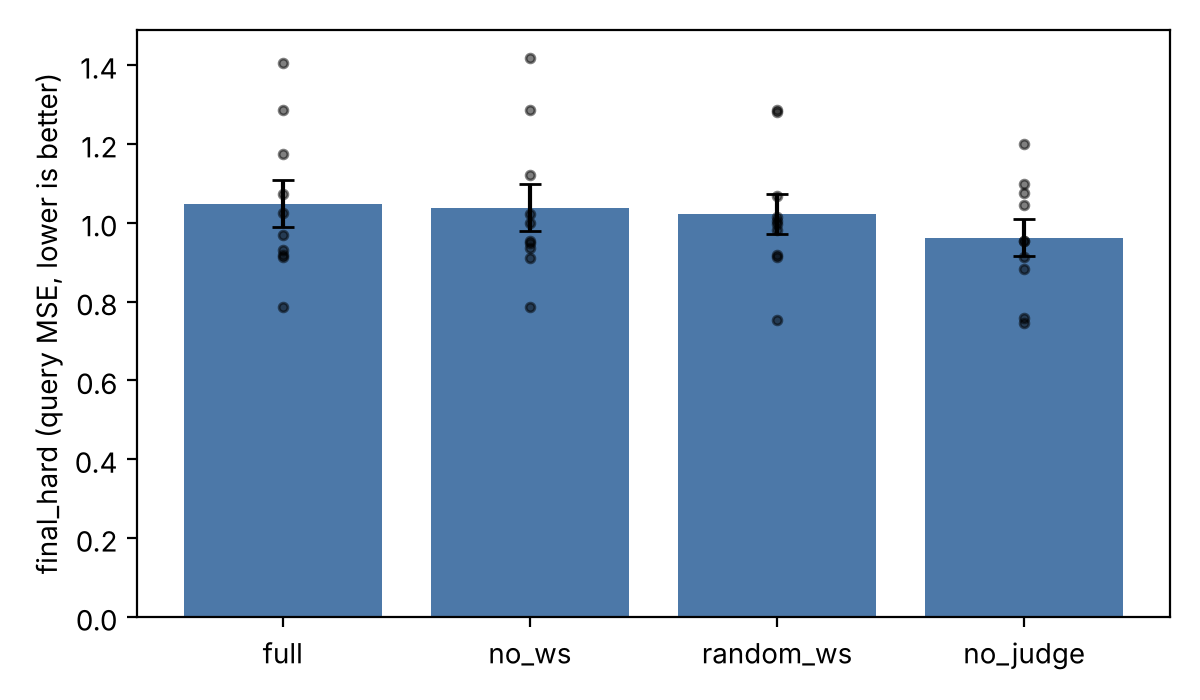
\includegraphics[width=0.62\linewidth]{results/final_hard.png}
\caption{\fh{} per arm: bars are means with standard errors, dots are individual seeds.}
\label{fig:fh}
\end{figure}

\begin{figure}[t]
\centering
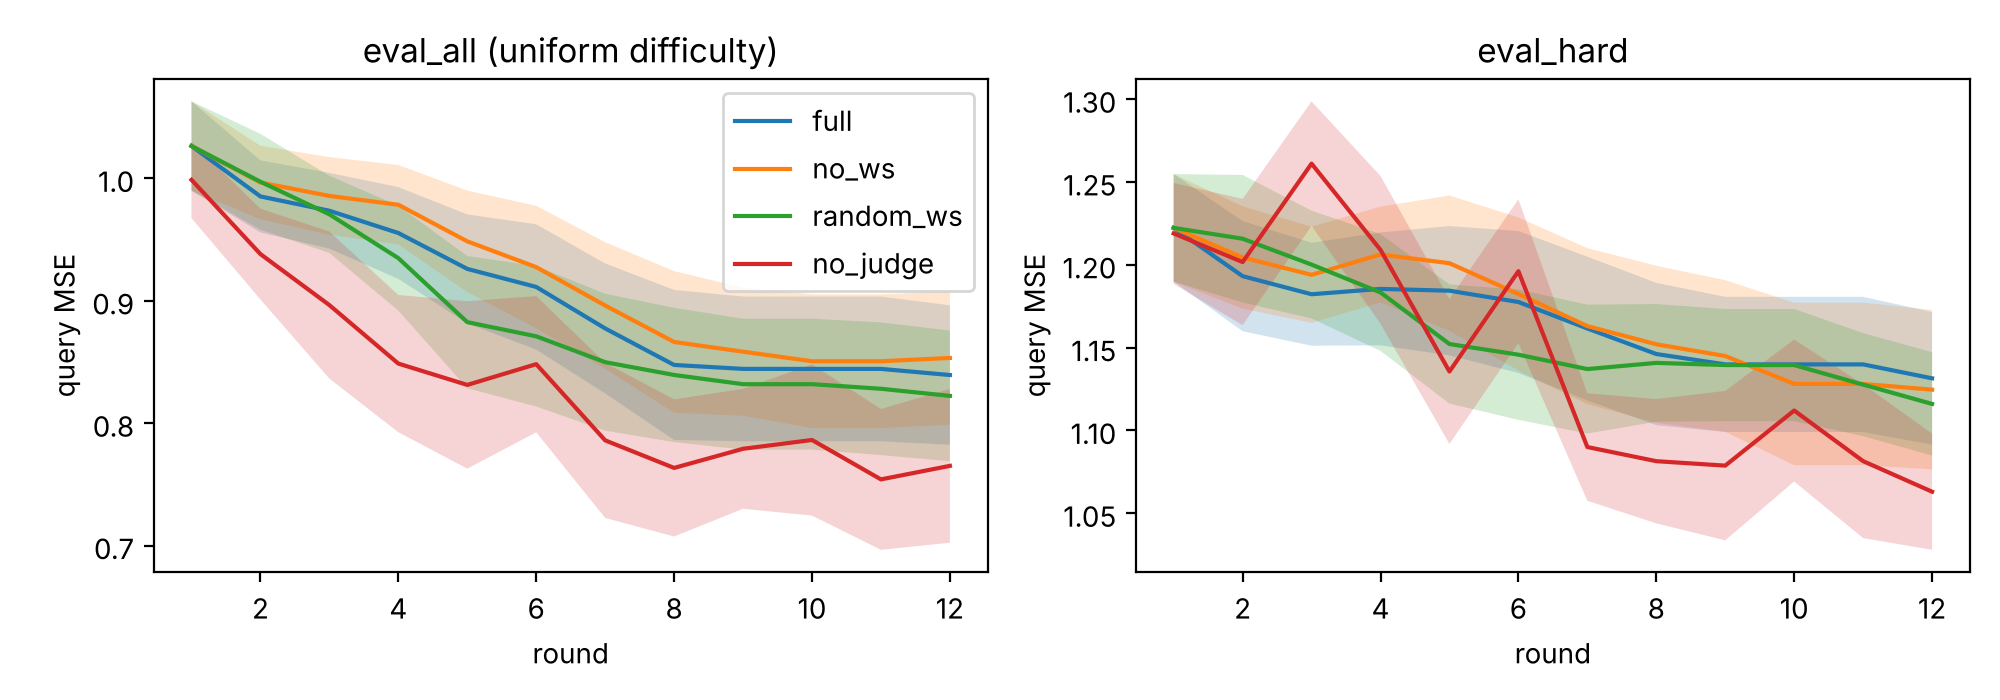
\includegraphics[width=\linewidth]{results/curves.png}
\caption{Per-round evaluation curves (mean $\pm$ s.e. over $10$ seeds) on a uniform-difficulty set (left) and the hard set (right).}
\label{fig:curves}
\end{figure}

\paragraph{H1 (competitive workspace vs.\ none): no detectable difference.} $\Delta=-0.010$ on \fh{}, Bonferroni CI $[-0.060,+0.034]$.
The interval is compatible with effects in either direction up to about $0.03$--$0.06$ and the approximate minimum detectable effect is $0.068$, above the SESOI.
This is \emph{not} evidence that the workspace has no effect.

\paragraph{H2 (competition vs.\ random winners): no detectable difference on the primary metric.} $\Delta=-0.027$, Bonferroni CI $[-0.071,+0.015]$; MDE $\approx0.061$.
On the secondary metric \auc{}, \texttt{random\_ws} was \emph{better} than \texttt{full} ($\Delta=-0.016$, 95\% CI $[-0.028,-0.005]$, Bonferroni CI $[-0.031,-0.003]$), a secondary, uncorrected-across-metrics
finding of unclear meaning that we do not interpret as an effect of workspace content. In one of ten seeds the three judged arms had identical \fh{}.

\paragraph{H3 (judge vs.\ no judge): the judge hurt in this toy.} \texttt{no\_judge} had lower \fh{} by $0.086$ (Bonferroni CI $[-0.168,-0.014]$), exceeding the SESOI; by the pre-specified rule the verdict is
``\texttt{full} clearly worse''. The effect is also present on \fa{} ($-0.117$) and \auc{}. \texttt{no\_judge} beat \texttt{full} on \fh{} in $8$ of $10$ seeds.
The mechanism is plausibly that the judge rejected about $73\%$ of rounds ($1-0.267$), so guarded arms retained roughly four times fewer accepted updates under an equal round budget;
the toy contains no adversarial optimization against the judge, so the benefit the guards are meant to provide cannot appear. We did not test this explanation.

\paragraph{H4 (Shapley interaction): the no-difference prediction was refuted, weakly.} In \texttt{full}, with round $0$ excluded, $9$ of $10$ seeds had both accepted and rejected rounds ($1$ dropped).
Mean $|I|$ was $0.0101$ on accepted and $0.0164$ on rejected rounds (difference $+0.0063$, 95\% CI $[+0.0019,+0.0110]$; signed difference $-0.0076$, CI $[-0.0133,-0.0020]$), not adjusted for multiplicity.
A larger magnitude on rejected rounds is confounded: rejected candidates may simply lie farther from the last accepted model, and the effect size is tiny relative to the loss scale.

\paragraph{Exploratory (not pre-registered).} The correlation between $\varphi_A$ and the judge's lower confidence bound across rounds of \texttt{full} was $0.73$ (partly mechanical, as both measure improvement of $A$-containing candidates).
Among $23$ accepted rounds (round $\ge1$), $2$ had worse \texttt{eval\_all} than the previous round. Mean accepted rounds per \texttt{full} seed: $3.2$ of $12$ (per-seed $4,1,3,2,6,4,2,4,4,2$).

\section{Discussion and Limitations}

\paragraph{Over-conservative judge.} On dev seeds the accept rate of \texttt{full} was $0.17$ ($83\%$ of rounds rejected); on report seeds it was $0.267$ ($\approx73\%$ rejected).
The gap monitor is anchored to the round-0 generalization gap (updated only on accepted rounds), so ordinary learning progress is flagged as overfitting; on dev seeds it flagged about $75\%$ of rounds even in \texttt{no\_judge}.
Even disabling it left a dev accept rate of $0.33$, so the lower-confidence-bound gate and the canary are also strict at this sample size. This is a design flaw we chose to report instead of tuning away; a recalibrated judge requires a new pre-registered study.

\paragraph{Curriculum collapse.} On dev seeds the curriculum concentrated on easy bins (hard-bin share $\approx0.02$ or lower by the last round), and all arms ended close to the zero-predictor level ($\approx1.29$) on the hard set (\fh{} between $0.96$ and $1.05$ on report seeds).
The toy therefore barely learns hard tasks at this budget, which limits the power of every comparison and of H1 and H2 in particular.

\paragraph{Boundary conditions.} (i) Synthetic regression with a non-learned, exact-ground-truth judge: no judge hacking can occur, so H3 says nothing about learned judges.
(ii) The workspace carries random projections of scalar statistics, not semantic content; null workspace results here do not transfer to LLM workspaces.
(iii) First-order meta-gradients; Shapley attribution covers $A$ and $B$ only.
(iv) Ten seeds and low power: confidence intervals are wide relative to the SESOI for H1 and H2.
(v) The pre-registration is informal and the dev seeds were inspected before the report run; no tuning followed, but readers should weigh this accordingly.
(vi) The word ``self-improvement'' denotes the loop's design; no open-ended or recursive improvement was observed or claimed.

\section{Conclusion and Reproducibility}

In a toy loop, a competitive workspace was not distinguishable from no workspace or a random workspace, and conservative judge controls reduced final accuracy relative to accepting every round,
mainly because they rejected most updates. The most useful outputs are methodological: an over-strict acceptance gate is itself a failure mode that must be calibrated before judging its benefits;
a pre-specified analysis plan with SESOI and Bonferroni intervals avoided over-reading small differences; and several silent bugs (identical arms due to the broadcast timing, divergence) were caught only by smoke tests.

\paragraph{Reproducibility.} Code and data: \repo. Hypotheses and dev-diagnostics commit: \commitHyp; frozen-config tag: \commitFrozen; results commit: \commitResults.
Verify \texttt{shasum -a 256 si\_loop\_toy.py run\_parallel.py} and the pre-run hypotheses (\texttt{git show <hypotheses-commit>:docs/hypotheses.md | shasum -a 256}) against Table~\ref{tab:hash}. Reproduce with
\texttt{python run\_parallel.py --seeds 1 2 3 4 5 6 7 8 9 10 --out results/ablation.json} followed by \texttt{python -I analyze.py results/ablation.json --out results/}.
Bit-exact reproduction may depend on the PyTorch version and platform.

\paragraph{AI assistance disclosure.} The code, the analysis scripts, the dev-seed diagnostics, and the drafting of this report were produced with substantial assistance from an AI system (Anthropic's Claude), under the author's direction.
The author decided the study design and the publication of null and negative results and is responsible for the content. All numerical values in this paper were checked programmatically against \texttt{results/analysis.json}.

\bibliographystyle{plainnat}
\bibliography{references}

\end{document}
